\documentclass[../main.tex]{subfiles}

\begin{document}

\subsection{Estructura del sistema}
Comenzaremos la sección de desarrollo dando contexto y mostrando la estructura del sistema, su arquitectura (véase \ref{fig:architecture_diagram}) y los patrones de diseño que se han seguido durante su desarrollo. Posterior a esta
sección, profundizaremos sobre los distintos componentes que contiene el sistema.

\begin{figure}[H]
\centering
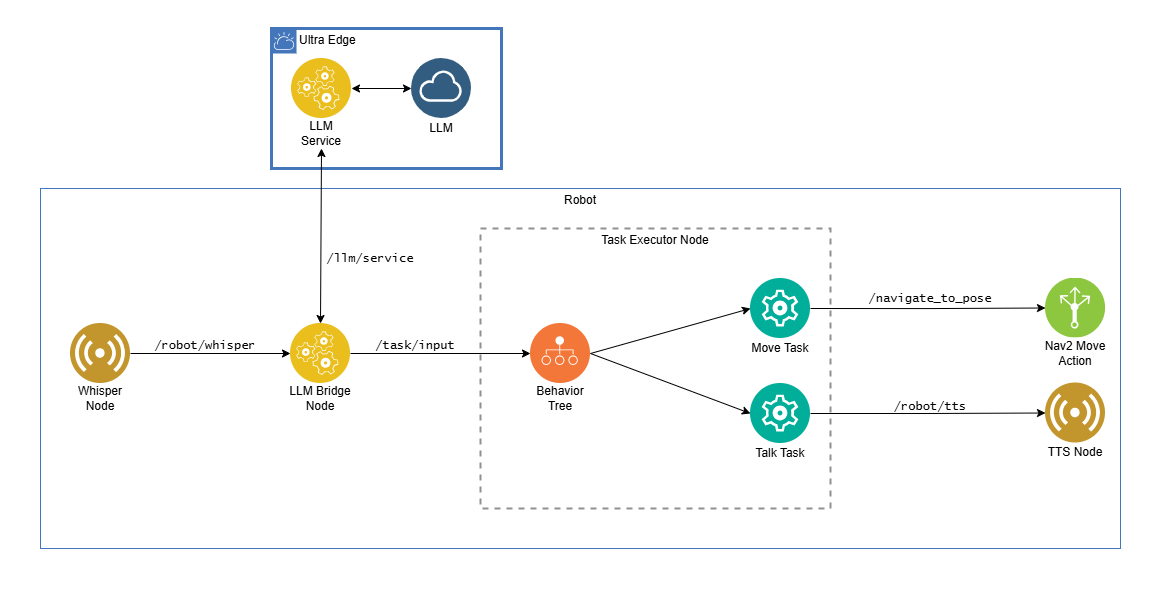
\includegraphics[width=\textwidth]{images/architecture.png}
\caption{Diagrama de la arquitectura y sus comunicaciones}\label{fig:architecture_diagram}
\end{figure}

\subsection{Sistemas de comunicaciones}
En este apartado del desarrollo abordaremos los sistemas de comunicaciones que se han implementado tanto para comunicarse los nodos de ROS2 entre sí como la integración
de un LLM como un servicio de ROS2

\blindtext

\subsection{Ejecutor y planificador de tareas}
\blindtext

\subsection{Integración con el robot físico}
\blindtext

\subsection{Interfaces gráficas para monitorización}
\blindtext

\end{document}